\documentclass[11pt]{article}
\usepackage{kotex}
\usepackage{amsfonts}
\usepackage{graphicx}

\def\logo{caulogo}

\begin{document}

\title{\begin{Huge}{How to use the the uility of git}\end{Huge}} 
\author{ChoiBowon}
\maketitle
\begin{center}\vspace{10mm}
\includegraphics[scale=0.5]{caulogo.png}\end{center}

\begin{flushleft}
\vspace{25mm}
창의ICT공과대학 소프트웨어학부 \\학번 20155212 \\성명 최보원 \\Git 주소 : https://github.com/ChoiBowon/assignment01
\end{flushleft}

\newpage
\tableofcontents

\newpage
\section{Git에 대한 간단한 정의?}
\begin{center}
\includegraphics[scale=0.1, width=1in]{gitlogo.png}\end{center}
	\subsection{버전 관리 소프트웨어}
	
	코딩과 관련된 개발 툴이다? 전혀 아니다. 
	
	Git은 페이스북과 플리커와 같은 소셜네트워크처럼 사용자가 자신의 프로필을 만들고 공유할 프로젝트를 올리며, 다른 계정을 팔로우 하여 소통도 가능하다. 주 목적이 프로젝트 개발자들의 소통이라고 보면 쉬울 것이다. 예로, 한 프로젝트에 대해 두 명의 개발자가 동시에 같은 부분을 수정한다고 하자. 각자 변경 사항을 업로드 할 경우 누군가의 작업은 겹쳐 쓰여지고 지워질 수 밖에 없을 것이다. 하지만 Git은 이 두 명의 변경 사항을 각각 저장하며 나중에 합쳐지는 과정에서도 그 어떤 작업도 잃어버리지 않고 병합할 수 있게 한다. 그리고 아래의 '스냅샷' 개념으로 이전 시점 즉, 어떠한 변화가 일어난 시점으로 되돌릴 수 있다.

	\subsection{스냅샷}

	기억해야 하는 중요한 점은 "스냅샷"이다. Git은 현재 추적하고 있는 프로젝트의 변화를 파일 단위로 기억하는 것이 아니다. 변화가 이루어진 그 순간을 중요하게 여기기 때문에 변화가 일어난 파일을 새로 저장하지 않고, 단지 이전 상태의 파일에 대한 링크만을 저장한다. Git이 데이터를 순간을 저장한 스냅샷의 스트림으로 취급한다는 것이다. 

	\subsection{빠른 속도}

	Git 이 서버, 즉 \textit{remote}(원격저장소)에도 프로젝트의 히스토리를 기억하고 있지만, Git 사용자는 대부분의 명령을 로컬 파일과 데이터에만 사용하기 때문에 네트워크가 필요 하지 않고, 이러한 이유로 속도가 빠를 수 밖에 없다. 예를 들면 사용자가 Git이 추적하고 있는 해당 프로젝트의 히스토리를 조회하고자 하면 Git은 서버를 거치지 않고 로컬단에서 조회를 하여 결과를 사용자에게 제공한다. 따라서, 파일을 비교하기 위해 \textit{remote}에 있는 서버에 접근하여 예전 버전을 갖고 오는 일이 필요가 없는 것이다. 

\newpage
\section{Git의 기능 적용}
	본인 소유의 컴퓨터에 실제로 적용하는 과정을 나열하도록 한다. 
	\subsection{git init}
	\begin{center}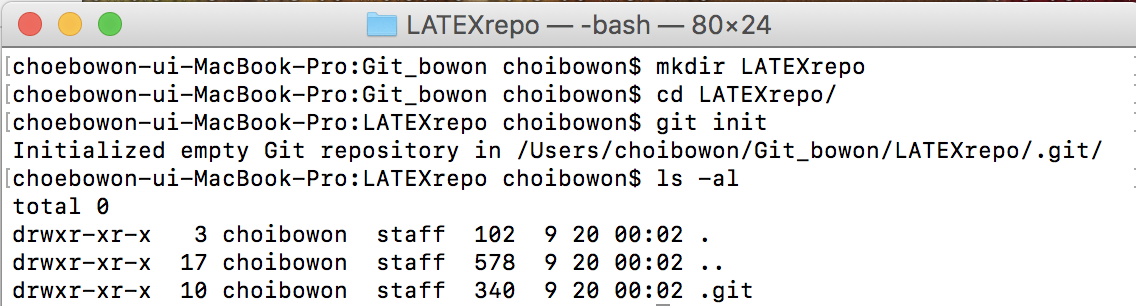
\includegraphics[width=5in]{gitinit.png}\end{center}
	choibowon 경로의 Git\_bowon 폴더 안에 \textbf{LATEXrepo} 라는 이름의 새로운 폴더를 \textit{mkdir} 명령어를 통해 생성한다. 위 그림의 .git을 통해 해당 폴더에 git initializion이 된 것을 확인 할 수 있다. 이 과정을 통해 LATEXrepo 는 로컬 저장소가 되는 것이다.
	
	\subsection{git remote}
	\begin{center}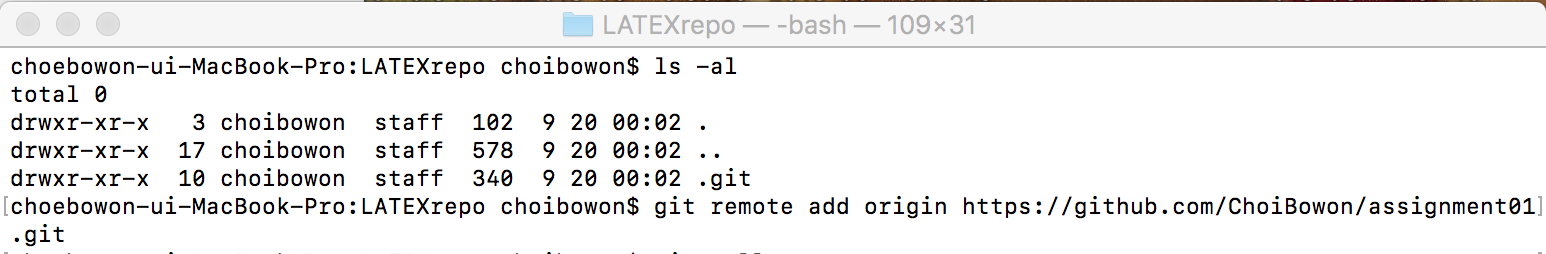
\includegraphics[width=5in]{gitremote.png}\end{center}
	LATEXrepo라는 이름의 내가 만든 로컬저장소와 github에 생성한 내 repository 를 담은 원격저장소(\textbf{assignment01})를 연결하기 위해 \textit{remote} 명령어를 이용한다.
	
	\begin{center}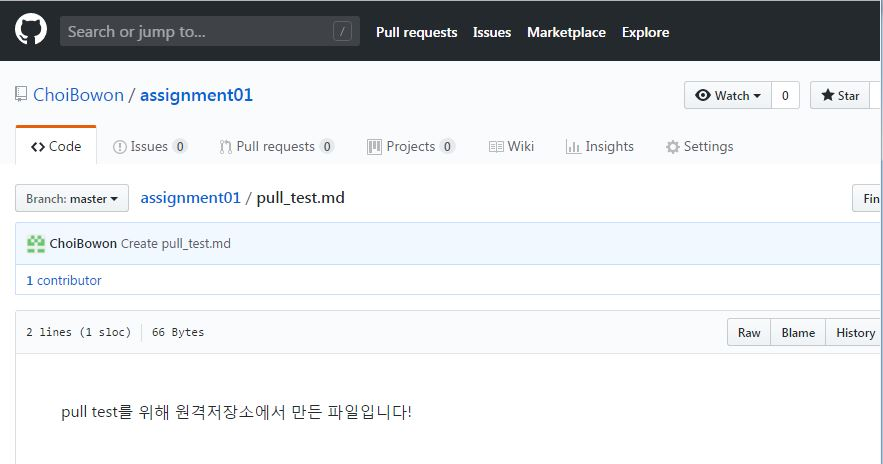
\includegraphics[width=5in]{pulltestremote.jpg}\end{center}
	위 화면은 원격 저장소와 로컬 저장소를 연결 한 후, 연동을 확인하기 위해 원격 저장소에 임의로 \textbf{pull\_test.md}라는 파일을 만든 것을 보여준다.
	
	\subsection{git pull}
	\begin{center}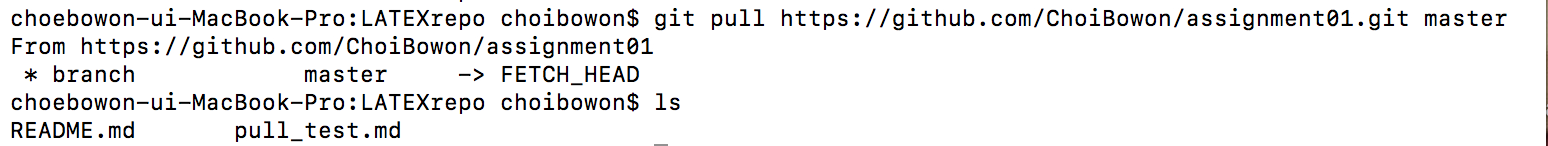
\includegraphics[width=5in]{gitpull.png}\end{center}
	로컬 저장소에서 \textit{git pull} 명령어를 실행하였더니 원격 저장소의 pull\_test.md 가 나타난다. 즉, 로컬과 원격저장소의 연동이 성공한 것이다.
	
	\begin{center}
\includegraphics[width=5in]{vimpulltest.png}\end{center}
	\begin{center}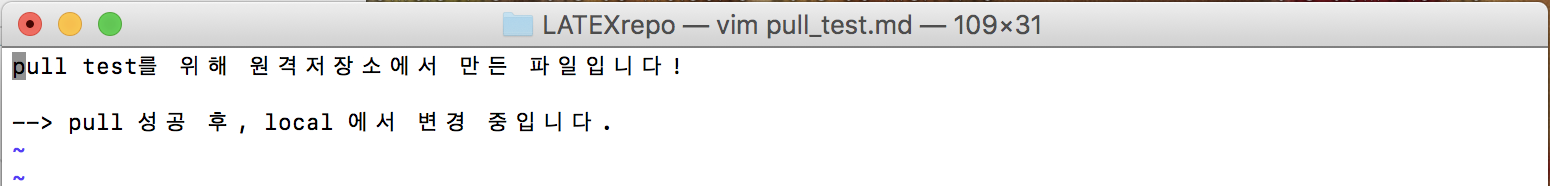
\includegraphics[width=5in]{pulltestrevision.png}\end{center}
	그리고 이번에는 로컬 저장소에서의 수정 사항이 원격 저장소에 잘 반영되는지 확인을 위해 로컬의 pull\_test.md 파일을 \textit{vim} 명령어를 통해 열고, 수정한다.
	
	
	\subsection{git add, git status}
	\begin{center}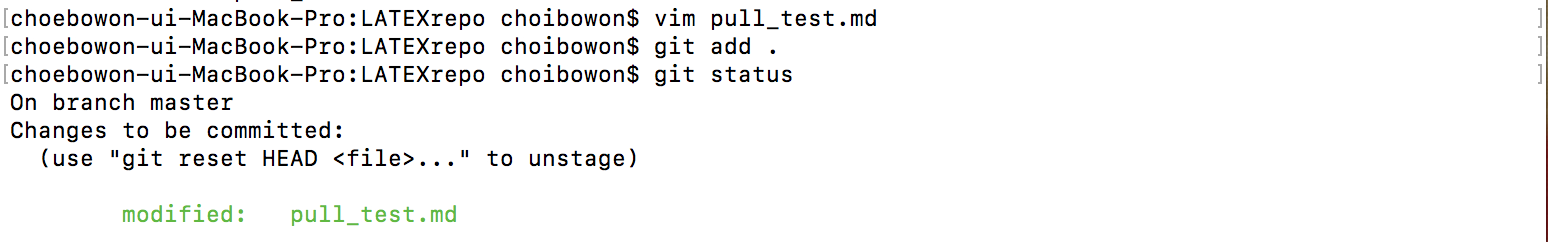
\includegraphics[width=5in]{gitadd.png}\end{center}
	\textit{git add} 명령어는 두 가지의 역할을 한다.
	\\\textbf{1.} untracked files 의 파일들을 git 이 추적하도록 한다.
	\\\textbf{2.} 파일은 수정했지만 아직 staging 영역에 올라가지 않은 'Changed but not updated' 파일들을 staging 영역에 올린다.
	
	위의 화면에서는 2번의 역할을 한 것으로, 이미 추적하고 있는 putt\_test.md 파일을 수정하고, 이것을 원격 저장소에 올릴 수 있도록 staging 영역에 올린 것이다. \\\textit{git status} 명령어는 현재 commit 되지 않은 변경사항을 조회하는 명령이므로, 이것을 실행한 결과 '\textbf{modified}'로 변경만 된 상태라는 것을 알려주는 것을 볼 수 있다.
	\\여기서 Git 에서 파일을 세 가지 상태로 관리하는 것을 언급하고자 한다. 
	\begin{itemize}\item Committed 란 데이터가 로컬 데이터베이스에 안전하게 저장되었다는 것을 의미한다. 
	\item Modified 란 수정한 파일을 아직 로컬 데이터베이스에 commit하지 않은 것을 의미한다.
	\item Staged 란 현재 수정한 파일을 곧 commit 할 것이라고 표시한 상태를 의미한다. 
	\end{itemize}
	
	\subsection{git commit, git push}
	\begin{center}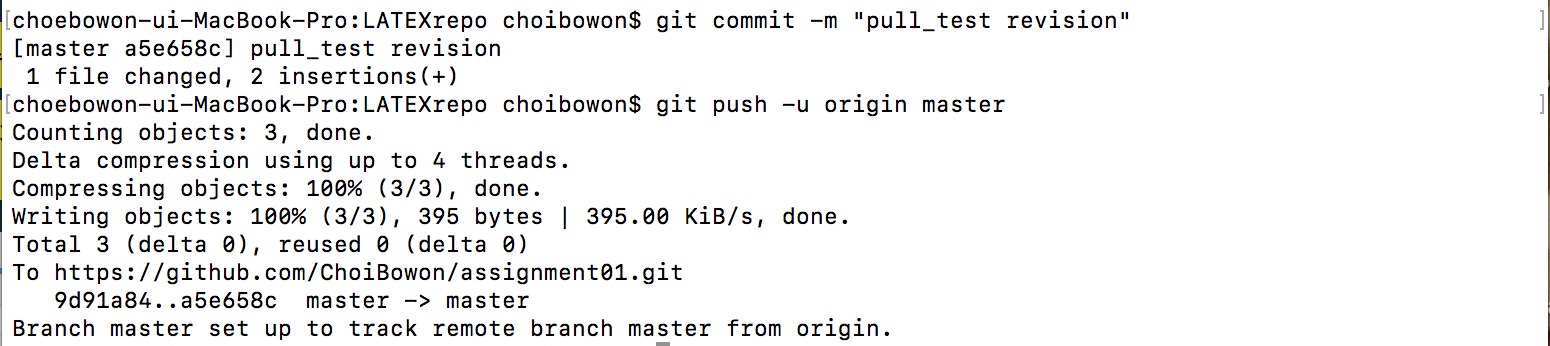
\includegraphics[width=5in]{gitcommitpush.png}\end{center}
	\begin{center}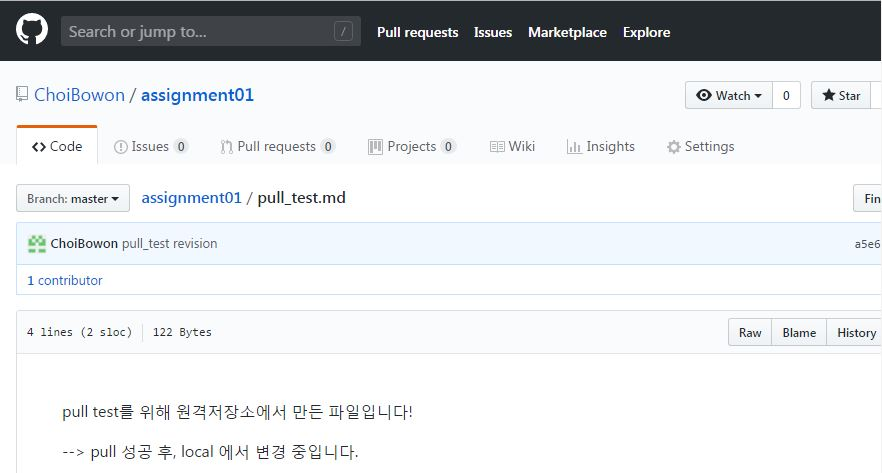
\includegraphics[width=5in]{pulltestlocal.jpg}\end{center}
	\textit{git commit} -m "commit message" 가 commit 명령어를 쓰는 형태이다. 이는 staging 영역에 올라가 있는 파일들을 commit 하는 것이며 -m 은 commit message 를 주는 옵션이다. 
	\\\textit{git push} 는 특별한 파라미터를 주지 않으면 원격 저장소, origin 저장소에 pushing한다. 
	
	\subsection{git branch}
	\begin{center}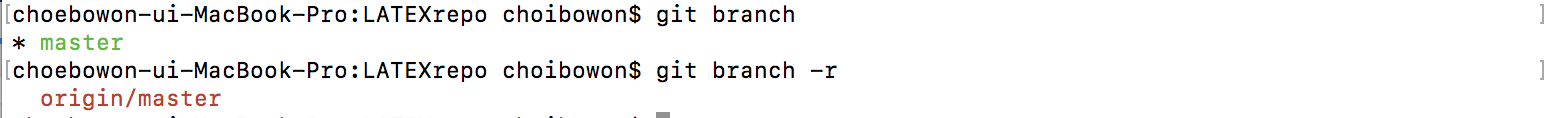
\includegraphics[width=5in]{gitbranch.png}\end{center}
	\textit{git branch} 명령어를 입력하면 현재 로컬의 브랜치를 보여주며, \textit{git branch -r} 을 입력하면 원격 저장소의 브랜치를 보여준다. 
	
	\subsection{git branch 브랜치명}
	\begin{center}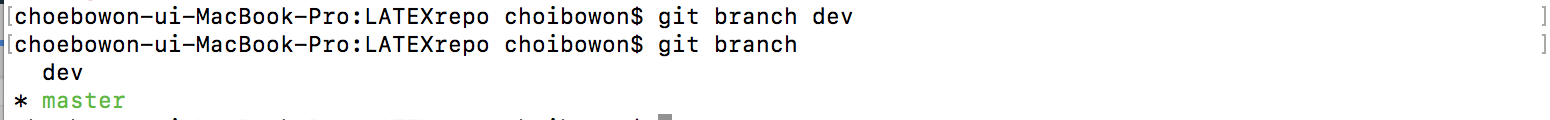
\includegraphics[width=5in]{createlocalbranch.png}\end{center}
	로컬에서 새로 브랜치를 생성하고자 하면 위처럼 기존의 \textit{git branch} 명령어 옆에 생성하고자 하는 브랜치의 이름을 적어주면 된다. \textbf{dev} 라는 이름의 브랜치를 생성한 것을 확인 할 수 있다.
	
	\subsection{git checkout 브랜치명}
	\begin{center}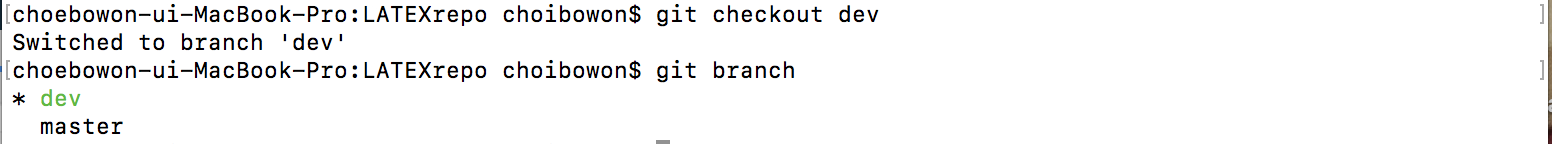
\includegraphics[width=5in]{changebranch.png}\end{center}
	dev 브랜치를 생성하였지만 아직 dev를 가리키고는 있지 않는 상황이다. dev에서 개발을 진행하고 싶다면 \textit{git checkout} 명령어를 통해 브랜치를 이동하여야 한다. 이동한 후, 다시 \textit{git branch}를 통해 확인하면 브랜치가 변경되었는지 확인 할 수 있다.
	
	\subsection{git push 브랜치}
	\begin{center}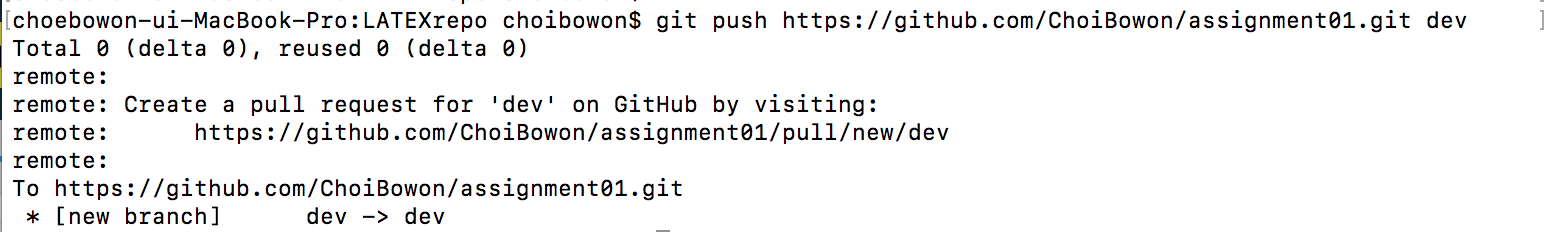
\includegraphics[width=5in]{branchtoremote.png}\end{center}
	\begin{center}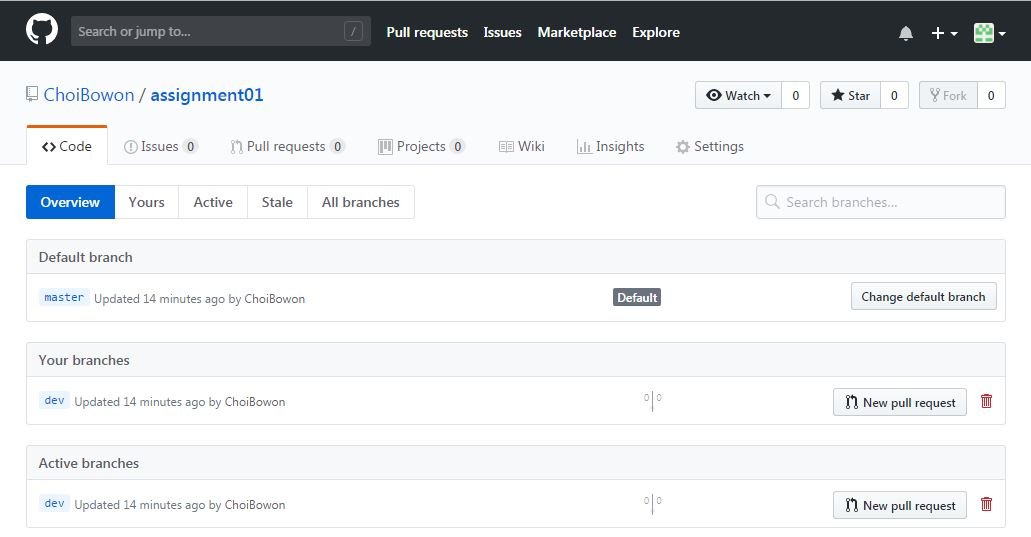
\includegraphics[width=5in]{createdev.jpg}\end{center}
	그럼 이제 로컬에서 생성한 브랜치가 원격 저장소에도 나타날 수 있게 해줘야 한다. 마찬가지로 \textit{git push} 를 통해 원격저장소로 전달한다. 그러면 아래 화면과 같이 원격 저장소에서 만들지 않았던 dev 라는 이름의 브랜치가 생성된다. 
	
	
	
	
	
	
\end{document}

